\documentclass{cpsc413Solutions}
\usepackage{amsmath}
\usepackage[utf8]{inputenc}
\usepackage{graphicx}
\graphicspath{{Images/}}
\usepackage{ dsfont }
\usepackage{ upgreek }
\usepackage{listings}

\coursetitle{Design and Analysis of Algorithms}
\courselabel{CPSC 413}
\exercisesheet{Problem Set \#[5]}{}
\student{Minh Hang Chu - 30074056}
\semester{Winter 2020}

\begin{document}

\team{Minh Hang Chu}

\sources{
Lecture Notes,
Algorithm Design textbook
}

\begin{problemlist}
\pbitem 
\begin{problem}
\begin{answer}

\begin{enumerate}
    \item Use the iteration method to come up with a good guess for a tight asymptotic bound for the recurrence.
    
    I use the tree method here since the instructor said that we can use any method.
    
    We have the tree as below:
    
    \begin{figure}[htp]
        \centering
        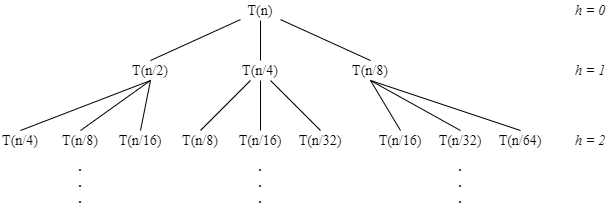
\includegraphics[width=15cm]{ProbSet5_1.png}
    \end{figure}
    
    We also assume that $n$ is the power of 2 so that we can drop all the floor.\\
    We can see that each recursive call of $T(p)$ has more $p$ steps.
    
    If $h=0$, the total cost is $n$.\\
    If $h=1$, the total cost is $\frac{n}{2}+\frac{n}{4}+\frac{n}{8}=\frac{7n}{8}=n\frac{7^1}{8^1}$\\
    If $h=2$, the total cost is $(\frac{n}{4}+\frac{n}{8}+\frac{n}{16})+(\frac{n}{8}+\frac{n}{16}+\frac{n}{32})+(\frac{n}{16}+\frac{n}{32}+\frac{n}{64})=\frac{49n}{64}=n\frac{7^2}{8^2}$.
    
    We can see that at level $h$, the total cost is $n\frac{7^h}{8^h}$.
    
    We make another assumptions here that all recursion trees have the same height.
    
    We need to compute the depth of the tree to find summation. We see that the lower bound with the smallest depth of the tree is $log_8(n)$ which will be the right-most branch the in tree above. Similarly, the upper bound with the depth of the tree is $log_2(n)$, at the left-most branch in the tree. Hence we have the sum for upper bound:
    $$\sum_{i=0}^{lg(n)}n\frac{7^i}{8^i}$$
    and for lower bound:
     $$\sum_{i=0}^{log_8(n)}n\frac{7^i}{8^i}$$
    
    We consider an asymptotic bound when $n \xrightarrow{}\infty$. Then both $lim_{n\xrightarrow{}\infty}log_8(n) = lim_{n\xrightarrow{}\infty}lg(n) = \infty$
    
    Then we have:
    $$lim_{n\xrightarrow {}\infty} \sum_{i=0}^{lg(n)}n\frac{7^i}{8^i}$$
    $$= lim_{n\xrightarrow {}\infty} (\frac{\frac{7}{8}^{lg(n)+1}-1}{\frac{7}{8}-1})$$
    $$= lim_{n\xrightarrow {}\infty} (-8) (-1)$$
    $$=8$$
    
    From here, we can guess that the tight asymptotic bound for $T(n)$ is $\Theta(n)$.
    
\newpage
    \item Prove that your guess is correct.
    Guess: the ceiling won't make any significant difference.
    
    We first show $T(n) \in O(n)$. We prove this by strong induction on $n$. 
    
    Choose $n_0 = 1$.
    
    \begin{itemize}
        \item
        Base case: $n \leq 8$.Then T(n) is bounded by a constant d. We choose $a \geq d$, which implies $T(n) \leq d \leq a \leq an$.
        
        \item Inductive Hypothesis: Let $k \in \mathds{Z}, k \geq 8$. Assume that $\forall m \in \mathds{Z},0\leq m \leq k,T(m) \leq am$.
        
        \item Inductive step: We want to show $T(k+1) \leq a(k+1)$. It is clear that $0 \leq \frac{k+1}{8} \leq \frac{k+1}{4} \leq \frac{k+1}{2} \leq k < k+1$.
        
        We have:\\
        $$T(k+1) = T(\lfloor\frac{k+1}{2}\rfloor) + T(\lfloor\frac{k+1}{4}\rfloor) + T(\lfloor\frac{k+1}{8}\rfloor) + (k+1)$$
        $$\leq a (\frac{k+1}{2}+\frac{k+1}{4}+\frac{k+1}{8}) + (k+1)$$
        $$= a (\frac{7(k+1)}{8})+(k+1)$$
        If $a (\frac{7(k+1)}{8})+(k+1) = a(k+1)$, we are done. Then we need to add $\frac{a}{8}(k+1)$ to a $a\frac{7(k+1)}{8}$ to get $a(k+1)$. Hence we choose $a\frac{k}{8}\geq k$ which means $a \geq \frac{8k}{k}= 8$. Then we pick $a = max \{d,8\}$. Thus:
        $$T(n) \leq a (\frac{7k}{8}+\frac{7}{8})+\frac{a}{8}(k+1)$$
        $$= a (\frac{7k}{8}+\frac{7}{8})+(\frac{ak}{8}+\frac{a}{8})$$
        $$= a(k+1)$$
        
        Hence, $T(n) \in O(n)$.\\
    \end{itemize}
    
    Now we need to prove that $T(n) \in  \Omega(n)$
    
    \begin{itemize}
       \item Base case: $n \leq 8$. Then $T(n)$ is lower bounded by a constant g.\\
       We pick $a \leq \frac{g}{n}$ then $an\leq g$ for this base case. Thus, $T(n)\geq g \geq an$. Then we let $a=g$
       
       \item Inductive Hypothesis: Let $k \in \mathds{Z}, k \geq 8$. Assume that $\forall m \in \mathds{Z},0\leq m \leq k,T(m) \geq am$.
       
       \item Inductive Step: We want to show $T(k+1) \geq a(k+1)$. It is clear that $0 \leq \frac{k+1}{8} \leq \frac{k+1}{4} \leq \frac{k+1}{2} \leq k < k+1$. 
       
        We have:\\
        $$T(k+1) = T(\lfloor\frac{k+1}{2}\rfloor) + T(\lfloor\frac{k+1}{4}\rfloor) + T(\lfloor\frac{k+1}{8}\rfloor) + (k+1)$$
        
        $$\geq a (\lfloor\frac{k+1}{2}\rfloor+\lfloor\frac{k+1}{4}\rfloor+\lfloor \frac{k+1}{8}\rfloor) + (k+1)$$
        $$\geq a (\frac{k+1}{2} -1 +\frac{k+1}{4} - 1 +\frac{k+1}{8} - 1) + (k+1)$$
        $$ = a(\frac{7(k+1)}{8}-3)+k+1$$
        $$=a(\frac{7(k+1)}{8}) + k +1 - 3a$$
        
       We want to get $a(k+1)$, we will need to add $-(k+1+3a) + (\frac{a}{8}(k+1))$ to $a(\frac{7(k+1)}{8})$. 
       
       Then we want $k \geq \frac{ak}{8}$ and $1-3a \geq \frac{a}{8}$. From here, we want $8 \geq a$ and $8-24a \geq a$.
       
       This implies that $8\geq a$ and $\frac{8}{25} \geq a$.
       
       We pick $b = min \{g,8,\frac{8}{25} \}$ so it will be satisfied that $k+1+3a \geq \frac{b}{8}(k+1)$.
       
       Thus we get:
       
       $$T(k+1) = b(\frac{7(k+1)}{8}) +k +1-3b$$
       $$\geq b(\frac{7(k+1)}{8} + \frac{b}{8}(k+1) $$
       $$= b(k+1)$$
       
       This implies that $T(n) \in \Omega(n)$.
       
       Since $T(n) \in O(n)$ and $T(n) \in \Omega(n)$, we can conclude that $T(n) \in \Theta(n)$.
       
    \end{itemize}
        
\end{enumerate}

\end{answer}
\end{problem}

\pbitem [Use the Master Theorem to abtain asymptotic bounds on recurrences]
\begin{problem}
\begin{answer}
We use Master Theorem definition on the slides. I'm not rewriting them here.
\begin{enumerate}
    \item $T(n) = 2T(\frac{n}{2})+n^3$
    
    $b = 2 \geq 1$, $a = 2 \geq 1$ and $f(n) = n^3$
    
    The third case is satisfied.
    
    We have: $n^{log_ba} = n^{log_2(2)}= n^1 = n$. Then we know that $f \in \Omega(n^{log_b(a)+\epsilon})$ for some $ \epsilon > 0$. If we pick $\epsilon = 2$, then we have $f(n) = n^3 \in \Omega (n^3)$.
    
    We also have: $af(n/b) = 2(\frac{n}{2})^3 = \frac{n^3}{4} \leq \frac{n^3}{2}  $. We pick $c = \frac{1}{2} < 1$. Then $af(n/b) \leq cf(n)$ and sufficiently large n.
    
    Thus, we get $T(n) \in \Theta(f(n)) = \Theta(n^3)$.
    
    \item $T(n) = 2T(\frac{n}{2})+n$
    
    $b = 2 \geq 1$, $a = 2 \geq 1$ and $f(n) = n$
    
    The second case is satisfied. 
    
    We have: $n^{log_b(a)} = n^{log_2(2)} = n^1 = n$. Then $f(n) = n \in \Theta(n)$ which is correct. Thus, we get: $T(n) \in \Theta(nlgn)$
    
    \item $T(n) = 2T(\frac{n}{2})+\sqrt{n}$
    
    $b = 2 \geq 1$, $a = 2 \geq 1$ and $f(n) = \sqrt{n} = n^{\frac{1}{2}}$
    
    The first case is satisfied.
    
    We have:  $n^{log_b(a)} = n^{log_2(2)} = n^1 = n$. Then $f(n) = \sqrt{n} \in O(n^{log_b(a) -\epsilon})$ which $\epsilon = 0.25$.
    
    Thus, we get: $T(n) \in \Theta(n)$.
    
    \item $T(n) = 4T(\frac{n}{8})+\sqrt{n}lg^2n$
    
     $b = 8$, $a = 4$ and $f(n) = 4T(\frac{n}{8})+\sqrt{n}lg^2n$
     
     The first case is satisfied. 
     
     We compute: $n^{log_b(a) = n^{log_8 4} = n^{2/3}}$. Then we have: $f \in O(n^{log_b(a) - \epsilon}$ for some $\epsilon > 0$. 
     
     We pick $\epsilon = \frac{1}{12}$. Since $lim_{n \xrightarrow{} \infty}\frac{\sqrt{n}lg^2n}{n^{7/12}}=0$, this implies $f \in o(n^{7/12} \longrightarrow f \in O(n^{7/12}$ 
     
     Thus, we get $T(n)\in \Theta(n^{2/3})$.
     
    
    \item $T(n) = 16T(\frac{n}{7})+n^2$
    
    $b = 7$, $a = 16 > 1$ and $f(n) = n^2$
     
     The third case is satisfied. 
     
     We compute: $n^{log_b(a)} = n^{1.424}$. We have $f(n) = n^2 \in \Omega(n^{log_b(a) + \epsilon})$ where $\epsilon = 2-log_7(16) > 0$, then we get $n^{log_7(16)+2-log_7(16)}= n^2$ and it is true that $f = n^2 \in \Omega(n^2)$.
     
     We also pick $c = \frac{1}{2}$, then we have: $af(\frac{n}{b}) = 16(\frac{n}{7})^2 = \frac{16n^2}{49} \leq \frac{1}{2}n^2 = cf(n) $.
     
     Thus, we get $T(n) \in \Theta(n^2)$.
\end{enumerate}

\end{answer}
\end{problem}

\pbitem [Let X and Y be two arrays, each containing n distinct integers in ascending order. The problem is to computer the median of all 2n elements in time $\Theta(lgn)$]

\begin{problem}
\begin{enumerate}
    \item Formal definition of the problem\\
    Precondition:
    \begin{itemize}
        \item Non-empty sorted arrays X, Y each has n integers in ascending order. 
    \end{itemize}
    
    Postcondition:
    \begin{itemize}
        \item Return an integer which is the median of 2n elements in X and Y. The median is the middle element of a sorted array. If there are 2 medians, we will pick the smaller median. 
        \item No side effects.
    \end{itemize}

\newpage    
    \item Give a divide and conquer algorithm to solve the problem
    
    \begin{lstlisting}[numbers=left, mathescape=true]
    findMedian(X,Y)
    if (X.size <= 2) then
        Z = mergeAscending(X,Y) // merge X and Y in ascending order
        return $Z[\lfloor(Z.size()-1)/2\rfloor]$ // return median of Z
    end if
    medianX = $X[\lfloor(X.size()-1)/2\rfloor]$
    medianY = $Y[\lfloor(Y.size()-1)/2\rfloor]$
    if (medianX = medianY) then
        return median X
    else if (medianX < medianY)
        newX = partition (X, $\lfloor (n-1)/2\rfloor$, X.size()-1)
        newY = partition (Y, 0, $\lfloor (n-1)/2\rfloor$)
        return findMedian(newX, newY)
    else // (medianX > medianY)
        newX = partition (X, 0, $\lfloor (n-1)/2\rfloor$)
        newY = partition (Y, $\lfloor (n-1)/2\rfloor$, Y.size()-1)
        return findMedian(newX, newY)
    \end{lstlisting}
    
    The function $partition (A,x,y)$ returns a part of list $A$ from index x to index y. 
    
\newpage
\item Prove that your algorithm is correct

We prove by induction on size of X and y. Let $n$ is the size of list X or Y.

Base case: $n \leq 2$. 

Line 3 is executed, merging 2 lists $X$ and $Y$ with elements in X and Y sorted in ascending order . $Z$ will have 2n elements.

Line 4 returns the median of R by finding the median index.

Inductive Hypothesis: Let $k \in \mathds{Z}, k \geq 2$. Suppose that for all integers $m$ so that $1 \leq m \leq k$, the algorithm is correct for any $X,Y$ with size $m$.

Inductive Step: We prove the algorithm is correct for $n = k+1$.

The execution will go to line 6. We compute median values of $X$ and $Y$ by returning number at median index. Median index is calculate at $\lfloor (size-1)/2 \rfloor$.

We denote $Z$ is the a list of all elements in X and Y in ascending order.

We compare this 2 medians, there are 3 cases.

\begin{itemize}
    \item $medianX = medianY$
    
    We know that X and Y has the same size. There are are $\lfloor(n-1)/2\rfloor$ elements of X that is less than $medianX$ and elements of Y less than $medianY$. Hence the maximum number of elements less than $medianX = medianY$ is $n-1$. Similarly, there are $n-1$ elements in X and Y that is greater than $medianX=medianY$.
    
    Since X and Y has n distinct elements, if we merge X and Y together with elements in ascending order, we will have 2 same elements as $medianX=medianY$ in Z. This 2 elements will be places right next to each other in the middle of the array $Z$. Let's assume that $medianX$ is positioned left of $medianY$.
    
    If $n$ is odd, there are $n-1$ elements are on the left of $medianX$ and $n-1$ elements positioned right of $medianY$. $Z$ has 2n elements The median of $Z$ is at $Z[n-1]$ position which is $medianX$.
    
    If $n$ is even, there are $n-2$ elements on the left of $medianX$ and $n$ elements on the right of $medianY$. $Z$ has 2n elements and the median index will be $n-1$ position. This means the median of $Z$ is will be at $Z[n-1]$ which is $medianY$. Since $medianX=medianY$, which is the median of $Z$.
    
    \item $medianX < medianY$
    
    Denote: $X = [x_0,x_1, \dots, x_{m-1},x_m, x_{m+1}, \dots , x_{n-1}]$ and $Y = [y_0,y_1, \dots, y_{m-1},y_m, y_{m+1}, \dots , y_{n-1}]$ where $x_m = medianX, y_m = medianY$. 
    
    Since $x_m < y_m$, the median must be in $x_{m}, \dots x_{n-1}$ or $y_0, \dots, y_m$. 
    
    \begin{itemize}
        \item Suppose the median is in $x_0, \dots, x_{m-1}$, denote $x_i$.
        \item We see that $x_i < x_m < y_m < y_{m+1} ... < y_{n-1}$. This implies that $x_i$ is less than at least $(\lfloor(n-1)/2\rfloor)+1$ elements. 
        
        \item We also know that $x_i< x_m < x_{m+1} < \dots < x_{n-1}$, this shows that $x_i$ is also less than at least another $(\lfloor(n-1)/2\rfloor)+1$ elements.
        
        Hence $x_i$ is less than at least $n+1$ elements, which means there are at least $n+1$ elements on the right of $x_i$, which indicates that $x_i$ is not the median of Z.
        
        Thus, the median is not in $x_0, \dots, x_{m-1}$.
        
        \item Similarly, suppose the median is in $y_{m+1}, \dots, y_{n-1}$, denote $y_i$. 
        
        \item We see that $x_0< \dots < x_m < y_m < y_i$. This means there are at least $(\lfloor(n-1)/2\rfloor)+1$ elements less than $y_i$.
        
        \item We also know that $y_0 < y_1 < \dots < y_m < y_i$. This shows there are $(\lfloor(n-1)/2\rfloor)+1$ elements that is less than $y_i$. 
        
        Hence, there are at least $n+1$ elements are smaller than $y_i$, which shows that $y_i$ cannot be the median of $Z$.
        
        Thus, the median is not in $y_{m+1}, \dots, y_{n-1}$.
    \end{itemize}
    
    From the reasoning above, we can conclude that the median is in $x_{m}, \dots x_{n-1}$ or $y_0, \dots, y_m$.
    
    Now in the algorithm, we want to take the part on the right of the medianX from $x_m, \dots x_{n-1}$ and the part on the left of the medianY $y_0, \dots, y_{n-1}$, we recursively call the algorithm in smaller input size $n-\frac{n}{2}+1$. From here, using inductive hypothesis, we can get the return value is the median of $newX$ and $newY$.
    
    We need to that the median of $newX$ and $newY$ is also the median of $X$ and $Y$.
    
    \begin{itemize}
        \item Let $Z$ be a list of all elements in $X$ and $Y$ in ascending order. 
        
        $Z= \{a_1, b_1, \dots , x_m, \dots, y_m, \dots \}$
        
        \item We add $x_0, \dots, x_{m-1}$ in front of $x_m$ since all elements are smaller than $x_m$. We also add $y_{m+1}, \dots, y_{n-1}$ after $y_i$ since these are bigger than $y_i$. The size of $\{x_0, \dots, x_{m-1} \}$ and $y_{m+1}, \dots, y_{n-1}$ are the same
        
        \item We also know that we found the median between $x_m, \dots, y_m$ from inductive hypothesis. Then adding the same number of elements outside $x_m$ and $y_m$ will still imply that the median value should still be between $x_m$ and $y_m$. Since er are adding the same number of elements on both sides, the median of $Z$ is the same as the median between $x_m$ and $y_m$.
        
        \item Thus, the median between $x_m$ and $y_m$ is also the median of $Z$.
    \end{itemize}
    
    \item $medianX>medianY$
    
    This explaination is the same for the case $medianX < medianY$, we just switch X and Y.
    
    \end{itemize}
Thus, by induction, our algorithm is correct.

\newpage
\item Express the run-time of your algorithm as a recurrence relation.  Explain why your recurrence relation is correct.

The base case is when the size is less or equal 2. The run time for this base cse is a constant $c \in \mathds{R}$.

For the recursive cases, before the recursive call at line 13 and 17, we calculate the median and partition the new lists, this takes a constant number of steps $c_1$. 

These steps will go through line 6,7, check if condition at line 8, it will either go to line 9 or go to else if. When the execution reached line 10 or 14, it execute the similar process: partition the list and execute recursive call.

We recursively call $findMedian(newX,newY)$ with the size $n- \lceil \frac{n}{2} \rceil +1$.

We can express the run time of the algorithm with recurrence as follows:

\[
T(n) =
\begin{cases}
c & \text{if $n \le 2$}\\
T(n - \lceil \frac{n}{2}\rceil + 1) + c_1 & \text{otherwise}
\end{cases}
\]

\newpage
\item Prove a tight asymptotic bound on the run-time of your algorithm

We prove upper bound first:

Base case: $n \leq 2$. Then $T(n)$ is upper bounded by a constant $c$. 

We pick $a \geq c$, this implies $T(n) \leq c \leq a \leq algn$. We can choose $a=c$.

Inductive Hypothesis: Let $k \in \mathds{Z}, k \geq 2$. Assume that $\forall m \in \mathds{Z}, 0 \leq m\leq k, T(m) \leq algm $.

Inductive Step: We want to show that $T(k+1) \leq alg(k+1)$. It is trivial that $\frac{k+1}{2} < k <k+1$. We have:

$$T(k+1) = T(k+1 - \lceil \frac{k+1}{2} \rceil  +1)+d$$

$$= T (k+1-(\frac{k+1}{2}+1)+1)+d$$
$$= T(k+1-(\frac{k+1}{2}+1)+d$$
$$= T(\frac{k+1}{2})+d$$
$$\leq alg(\frac{k+1}{2})+d$$
$$=a(lg(k+1) - lg(2))+d$$
$$=alg(k+1) - a+d$$

We need to make $-a+d \leq 0$, then we can choose $a = max \{c,d \}$. We have:

$$T(k+1) \leq alg(k+1) -a+d$$
$$ \leq alg(k+1)$$

This shows that $T(n) \in O(lgn)$.

Next we prove lower bound, we know that $T_n = T(n - \lceil \frac{n}{2}\rceil + 1) + c_1 > T(\lceil \frac{n}{2}\rceil) +c_1 = T'(n)$.

We prove that $T'(n) \in \Theta(lgn)$, which will imply the lower bound for $T(n)$.

We use Master Theorem to prove lower bound. We use the second case here.

We get $a = 1, b=2, f(n) =c_1$.

Then we have $f(n) = c_1 \in \Theta(n^{log_2(1)})= \Theta(1)$, this implies $T'(n) \in \Theta(lgn)$.

Hence, $T(n) \in \Omega(lgn)$.

Since $T(n) \in O(lgn)$ and  $ T(n) \in \Theta(lgn)$, we can conclude that $T(n) \in \Theta(n)$.

\end{enumerate}
\end{problem}

\end{problemlist}


\end{document}
